\noindent The goal for this course is to explain the current "standard model" for particle physics. This is too lofty of a goal for this course, so what we focus on is the textit{building blocks} of the standard model, such that we understand the origin and purpose of each term of the Lagrangian. \\

\noindent Topics covered include

\begin{enumerate}
\item Path integral quantization
	\subitem Via Gaussian integrals.
\item Review perturbation theory via path integrals
	\subitem Includes familiar tools for calculating correlation functions such as Wick's theorem, Feynman rules, etc.
\item Renormalization
	\subitem Allows us to discuss effective QFT (e.g., eliminating infinities) in more detail.
\item Abelian and nonabelian classical gauge theories
	\subitem Uses path integrals to deduce quantizations from classical field theories.
\item Quantization of non-abelian gauge theories
	\subitem Employs path integrals for perturbative calculations and lattices for nonperturbative calculations.
\item Spontaneous symmetry breaking mechanisms
\end{enumerate}

\subsection*{Path Integrals}

\noindent Let's first suppose that the quantization is already done, and we have a quantum system with a Hilbert space $\mathcal{H}$, a Hamiltonian $\hat{H}$, and a propagator from integrating the Schroedinger equation, $U(t) = e^{-i\hat{H}t}$. \\

\noindent Now work out a representation to first order for the propagator by Taylor expanding

\begin{equation}
U(t) = e^{-i\hat{H}t} = \left( e^{-\frac{it}{N}\hat{H}}  \right) ^N= \lim_{N \rightarrow \infty} \left( \mathbb{I} - \frac{it}{N}\hat{H} \right) ^N
\end{equation}

\noindent Let $\{ \ket{j} \}$ be a basis for the Hilbert space $\mathcal{H}$ and consider the transition amplitude of evolving from an eigenstate $\ket{\phi_i}$ to another eigenstate $\ket{\phi_f}$

\begin{equation}
\bra{\phi_f} U(t) \ket{\phi_i} = \bra{\phi_f}  \left( e^{-\frac{it}{N}\hat{H}}  \right) ^N \ket{\phi_i}
\end{equation}

\noindent Insert  $N-1$ Hilbert space basis completeness relations, one in between each of the $N$ exponentials, and note that the sum over all paths from initial state to final state of functions of the paths

\begin{align}
\bra{\phi_f} U(t) \ket{\phi_i} &= \sum_{j_1,\dots,j_{N-1}} \bra{\phi_f} e^{-\frac{it}{N}\hat{H}} \ket{j_{N-1}}\bra{j_{N-1}} e^{-\frac{it}{N}\hat{H}} \dots \ket{j_1}\bra{j_1} e^{-\frac{it}{N}\hat{H}} \ket{\phi_i} \\
&\equiv \sum_{\text{paths}} f(j_1, \dots , j_{N-1}).
\end{align}

\noindent So, the transition amplitude of this state evolution is a sum over all of the paths through the basis states $j_1,\dots,j_{N-1}$. An example schematic of a path is visualized below.

\begin{figure}[H]
	\centering
	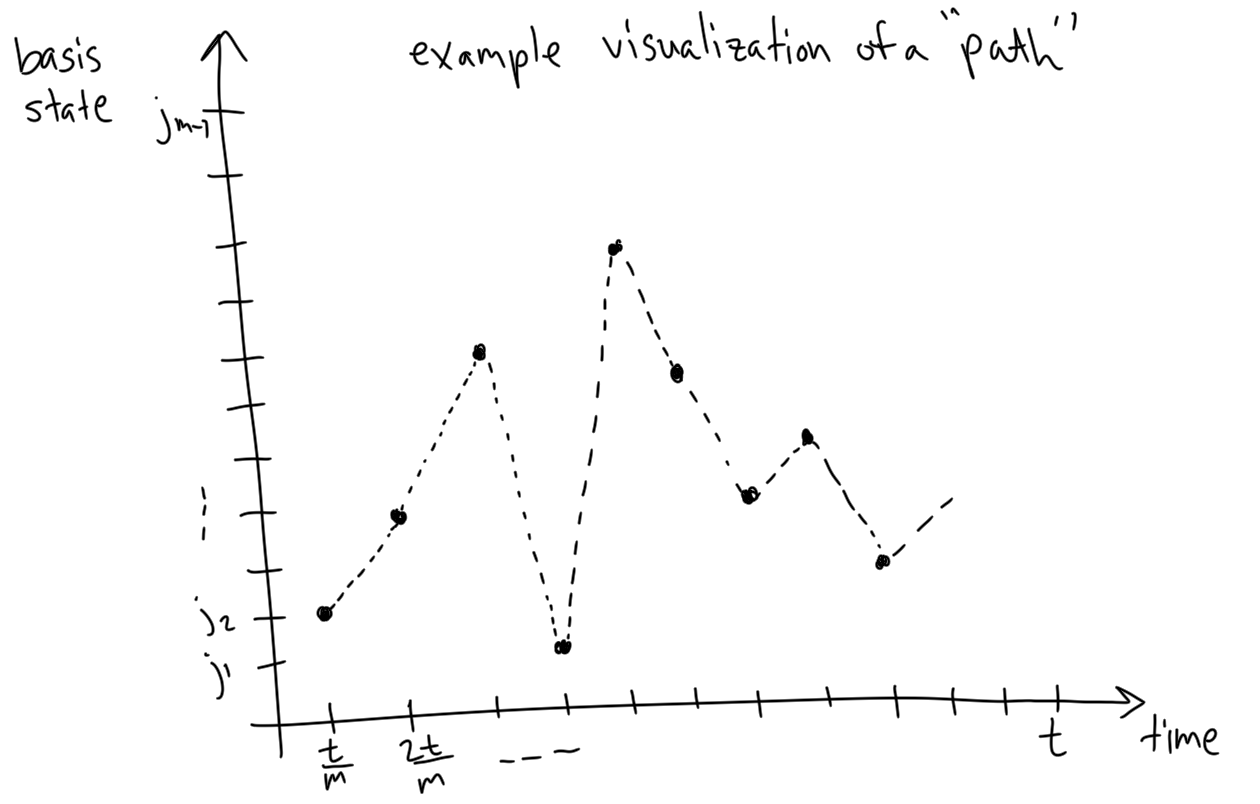
\includegraphics[width=4in]{images/pathviz.png}
	\caption*{}
\end{figure}

\noindent To work out the function of the path $f(j_1, \dots, j_{N-1})$, we need to calculate these individual transition amplitudes between successive states $\ket{j_{k-1}}$ to some final state $\bra{j_k}$ in the path integral setting, and seek to write it as an exponential of some function of the states $\mathcal{L}(j_{k-1}, j_k)$, the Lagrangian density

\begin{equation}
\bra{j_k} (\mathbb{I} - \frac{it}{N} \hat{H}) \ket{j_{k-1}} \simeq e^{\frac{it}{N} \mathcal{L}(j_{k-1}, j_k)}.
\end{equation}

\noindent So, the full transition amplitude will be a product of exponentials pf Lagrangian densities, well-known classical quantities

\begin{equation}
\bra{\phi_f} U(t) \ket{\phi_i} = \sum_{\text{paths}} f(j_1, \dots , j_{N-1}) = \sum_{j_1,\dots,j_{N-1}} e^{\frac{it}{N} \sum_{k=2}^{N-1} \mathcal{L} (j_{k-1}, j_k) } .
\end{equation}

\noindent Before moving forward, what makes the path integral so interesting?

\begin{enumerate}
\item It allows the calculation of quantum quantities, the transition amplitudes, via well-understood classical solutions and methods for handling highly oscillatory integrals such as the saddle point method.
\item It can also be used to build nonperturbative approximation schemes, such as Monte Carlo sampling over paths.
\end{enumerate}

\subsection*{Example: General Nonrelativistic Quantum Mechanical System}

\noindent Let's assume a little bit more about our quantum system. Suppose the quantum system is inspired by a classical system with pairs of canonical coordinates and momenta and the Hamiltonian $H(\{q^j\},\{p^j\}) = H(q,p)$. \\

\noindent Turn around the path integral sum over paths to guess a quantum Hamiltonian and Hilbert space from this classical Hamiltonian via

\begin{equation}
U(q_i, q_f, T) = \bra{q_f} U(T) \ket{q_i} = \bra{q_f} e^{-iT\hat{H}} \ket{q_i}
\end{equation}

\noindent Proceed as before, mulitplying the exponentials and inserting $N-1$ completeness relations in between the $N$ copies of the exponential. The completeness relation for the canonical position basis, a continuous variable, is

\begin{equation}
\mathbb{I} = \left( \prod_j \int dq_k^j \right) \ket{q_k} \bra{q_k}
\end{equation}

\noindent So, the transition amplitude in this case is, with $\epsilon \equiv \delta t = \frac{T}{N}$

\begin{equation}
\bra{q_f} U(T) \ket{q_i} = \sum_{k_1,\dots,k_{N-1}} \bra{q_f} e^{-i \epsilon \hat{H}} \ket{q_{k_{N-1}}} \bra{q_{k_{N-1}}} \dots \ket{q_{k_1}}\bra{q_{k_1}} e^{-i \epsilon \hat{H}} \ket{q_i}.
\end{equation}

\noindent There are three cases for the dependence of the quantum Hamiltonian on the canonical coordinates in the expression for the propagator. It can depend purely on position, purely on momenta, or most realistically, it can depend on both. \\

\noindent In the case that the Hamiltonian is a function purely dependent on canonical position, such that $\hat{H} = g(\hat{q})$, we easily calculate the transition amplitude, which relates the quantum and classical canonical positions, since the $\ket{q_k}$ are energy eigenstates of the position-dependent Hamiltonian

\begin{align}
\bra{q_{k+1}} g(\hat{q}) \ket{q_k} &= g(q_k) \prod_j \delta ( q_k^j - q_{k+1}^j ) \\
&= g \left( \frac{q_{k+1} + q_k}{2} \right) \left( \prod_j \int \frac{dp_k^j}{2\pi} \right) e^{ i \sum_j p_k^j (q_{k+1}^j - q_k^j ) }.
\end{align}

\noindent Where we used the Dirac delta distribution identity $\delta (q) = \int_{-\infty}^{\infty} \frac{dp}{2\pi} \, e^{i p \cdot q}$ to introduce the canonical momenta into the transition amplitude. Also note that the Dirac delta function forces $q_{k+1} = q_k$, such that $f(q_k) = f(\frac{q_{k+1} + q_k}{2})$, and we write it in this fashion for later use. \\

\noindent Next, in the case that the Hamiltonian is a function purely dependent on canonical momenta, such that $\hat{H} = h(\hat{p})$, the transition amplitude is calculated by inserting the completeness relation for the momentum eigenbasis.

\begin{align}
\bra{q_{k+1}} h(\hat{p}) \ket{q_k} &= \bra{q_{k+1}} h(\hat{p}) \cdot \prod_j \int dp_k^j \ket{p_k} \braket{p_k | q_k} \\
&= \prod_j \int \frac{dp_k^j}{2\pi} \, h(p_k) e^{ i \sum_j p_k^j (q_{k+1}^j - q_k^j ) }
\end{align}

\noindent Where the inner product of the position and momentum eigenstates is a Fourier phase element $\braket{p | q} = \frac{1}{2\pi} e^{i p \cdot q}$, and we get the sum, since the subscript $k$ denotes $N$ total canonical coordinate pairs. \\

\noindent The more realistic situation is when the Hamiltonian is dependent on both position and momenta $\hat{H} = \hat{H}(\hat{q}, \hat{p}) = g(\hat{q}) + h(\hat{p})$. Suppose the dependencies are linearly separable in the quantum Hamiltonian. Then we may translate between classical position and momenta via the Taylor expansion to first order

\begin{equation}
e^{-i \epsilon \hat{H}} = \mathbb{I} - i \epsilon \hat{H} = \mathbb{I} - i \epsilon (g(\hat{q}) + h(\hat{p})).
\end{equation}

\noindent Using this linearity, we can write this dependence in the derived formula as

\begin{equation}
\bra{q_{k+1}} e^{-i \epsilon \hat{H}(\hat{q}, \hat{p})} \ket{q_k} = \prod_j \int \frac{dp_k^j}{2\pi} \, e^{ -i \epsilon H (\frac{q_{k+1}+q_k}{2}, p_k)} e^{ i \sum_j p_k^j (q_{k+1}^j - q_k^j ) }
\end{equation}

\noindent Putting all this together into the propagator, which is really the transition amplitude for a nonrelativistic quantum system,

\begin{equation}
U(q_i, q_f; T) = \left(  \prod_{jk} \int dq_k^j \int \frac{p_k^j}{2\pi} \right) e^{i \sum_k \left( \sum_j p_k^j (q_{k+1}^j - q_k^j) - \epsilon H (\frac{q_{k+1} + q_k}{2}, p_k) \right)}.
\end{equation}

\noindent Take note that there is nothing quantum on the RHS: no hats! We have used purely classical data to define the quantum propagator, or, transition amplitude, on the LHS, such that $U(q_i, q_f; T) \propto e^{- i \epsilon H (q_i, q_f; T)}$. \\

\noindent A few other remarkable points:

\noindent Using the saddle point method, we can build an approximation scheme for $U$. This is useful for solving highly oscillatory integrals, as we see in the transition amplitude above (e.g., $e^{i\dots}$), since such integrals can be approximated by its saddle points (or critical points), which correspond to classical paths of the system. \\

\noindent Monte Carlo sampling of the system can also be used to approximate the transition amplitude by building an estimator for the RHS, sampling over classical configurations, and summing up the estimator. \\

\noindent Now, the expression for $U$ was not-so-pretty, but imagine continuous time variables and integrals when you see $\sum_k$ and $\epsilon$ above. In the limit as $N \rightarrow \infty$ (the number of completeness relations inserted), the quantum propagator is expressed in a continuous form with strange new "integrals".

\begin{equation}
U(q_i, q_f; T) = \left( \int \mathcal{D}q \int \mathcal{D} p \right) e^{i \int_0^T dt \, (\sum_j p^j \dot{q}^j - H(q,p))}
\end{equation}

\noindent Do not think of these as literal integrals, as we do not have a proper measure space to integrate over. Think of them as algorithms for now, something totally new that will be applied to solve this expression above.